% !TEX root = ../../main.tex

\chapter{Evaluation}
\label{chapter:evaluation-discussion}
This chapter presents Contribution \textbf{C.2}: A robust cost estimator for Amalur's factorized ML framework, and a comparison with the SOTA in \autoref{sec:eval-model-evaluation}. Prior to that, the methodology for collecting results is detailed in \autoref{sec:6experiment-setup}. The last section, \autoref{sec:eval-discussion}, offers a thorough analysis of the results and a critical perspective on the implications and constraints of this research.

\section{Experiment Setup}
\label{sec:6experiment-setup}
This section provides a comprehensive explanation of all the necessary steps to reproduce the results. It covers the experimental setup (\hyperref[subsec:6-software]{Software}, \hyperref[subsec:6-datasets]{Datasets} \& \hyperref[subsec:6-hardware]{Hardware}), as well as the data processing methods employed to guarantee reliable outcomes for the cost estimators (\hyperref[subsec:6-validation-strategy]{validation strategy}). For further details and implementations, please consult the GitHub repository\footnote{\url{https://github.com/ptemarvelde/amalur-experiments}}.

\subsection{Software}
\label{subsec:6-software}
The factorized ML framework (Amalur \cite{amalur}) is implemented in Python (3.10.4) and uses SciPy (1.8.0), NumPy (1.22.4) and CuPy (12.1.1). All experiments were run in a Docker container with an image based on Nvidia's base image with CUDA 12.1.1 and Ubuntu 20.04\footnote{\href{https://hub.docker.com/layers/nvidia/cuda/12.1.1-devel-ubuntu20.04/images/sha256-5bd13c67a4479a1c13238b470d89a92937ce68ba5f21b930d50c463e3314f657?context=explore}{nvidia/cuda:12.1.1-devel-ubuntu20.04}}.

The choice to use CuPy as the backend for the factorized ML framework was made to ensure that the experiments could run on both CPU and GPU. CuPy is a GPU-accelerated library for numerical computations that is compatible with NumPy and SciPy \cite{cupy_learningsys2017}. This allows for minimal changes to the codebase whether you are using a GPU or a CPU. To allow for exploitation of multiple cores for sparse matrix multiplication\footnote{\url{https://github.com/flatironinstitute/sparse_dot}} we use MKL (Intel Math Kernel Library) \cite{intel-mkl} as NumPy's backend for the CPU experiments.

For collecting the GPU metrics, we use NVIDIA's Nsight Compute (ncu)\footnote{\url{https://docs.nvidia.com/nsight-compute/NsightComputeCli/index.html}} which is a command-line profiling tool that collects detailed performance metrics from the GPU. The metrics are collected in a CSV file for downstream analysis, detailed in \autoref{sec:5-feature-engineering}. The cost estimators were created using Scikit-learn \cite{scikit-learn}.

\subsection{Datasets}
\label{subsec:6-datasets}
The datasets used in the experiments are a mix of synthetic and real-world datasets. The synthetic datasets are used to generate a training set to train the cost estimators on. The real-world datasets are used to validate the cost estimators on unseen data.

\subsubsection{Synthetic Datasets}
To create the synthetic datasets with a wide variety of data characteristics the data generator from \cite{schijndel_cost_estimation} was used, which in turn is an adaptation of the data generator\footnote{\url{https://github.com/delftdata/valentine-data-fabricator}} from \cite{valentine-data-generator}. In total, we generate $2415$ datasets, each being a two-table join. All other parameters were varied; the values are shown in \autoref{tab:6-synthetic-dataset-characteristics}.

\begin{table}[ht]
    \centering
    \begin{tabular}{llr}
        \toprule
        Data Characteristic             & Symbol    & Range                              \\ \midrule \midrule
        $S_1$ (Entity) table rows       & $r_{S_1}$ & $[ 40,000\text{,\ \ } 1,000,000]$  \\
        $S_2$ (Attribute) table rows    & $r_{S_2}$ & $[ 526\text{,\ \ } 1,000,000]$     \\
        $S_1$ (Entity) table columns    & $c_{S_1}$ & $[ 1\text{,\ \ } 50]$              \\
        $S_2$ (Attribute) table columns & $c_{S_2}$ & $[ 2\text{,\ \ } 50]$              \\
        Target table rows               & $r_T$     & $[ 60,000 \text{,\ \ } 1,000,000]$ \\
        Target table columns            & $c_T$     & $[ 11\text{,\ \ } 100]$            \\
        Target Sparsity                 & $e_T$     & $[ 0.0\text{,\ \ } 0.9]$           \\
        Tuple ratio                     & $\rho$    & $[ 1\text{,\ \ } 190]$             \\
        Feature ratio                   & $\tau$    & $[ 0.2\text{,\ \ } 1]$             \\
        Join Type                       & $j_T$     & Inner, left or outer.              \\
        Selectivity                     & $\sigma$  & $[ 1.0\text{,\ \ } 2.0]$           \\
        \bottomrule
    \end{tabular}
    \caption{Ranges of data characteristics for the generated synthetic datasets}
    \label{tab:6-synthetic-dataset-characteristics}
\end{table}

The data is organized in a star schema. $S_1$ is the Entity (transactional) table, which is connected to the attribute table $S_2$. This attribute table holds the features of the entities. The target table $T$ is the result of the join between $S_1$ and $S_2$. An example with an inner join is shown in \autoref{fig:6-data-gen-example}.

\begin{figure}
    \centering
    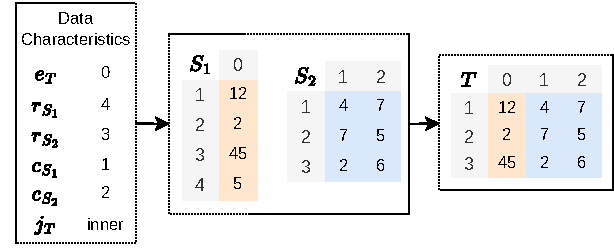
\includegraphics[width=0.8\linewidth]{chapters/06_evaluation/figures/data-gen-example.pdf}
    \caption[Example of generated synthetic dataset]{Example of synthetic dataset generation. The entity table $S_1$ is joined with the attribute table $S_2$ to create the target table $T$.}
    \label{fig:6-data-gen-example}
\end{figure}

\subsubsection{Real-world Datasets}
The synthetic datasets are convenient for testing and training purposes. However, in order to assess whether the cost estimators are generalizable to real-world data, we use real-world datasets for validation.

\paragraph{Project Hamlet \cite{2016-hamlet-sigmod}}
The Hamlet datasets are extensively used in the relevant literature \cite{2016-hamlet-sigmod, amalur, morpheus,orion_learning_gen_lin_models}. Comprising a collection of seven datasets, the Hamlet datasets are tailored to simulate data integration scenarios within a machine learning workflow. Initially developed to assess inner join scenarios, certain rows from various source tables were excluded to accommodate other join types. The data attributes of these datasets are detailed in \autoref{tab:6-hamlet-characteristics}.

\begin{table}[ht]
    \centering
    \begin{tabular}{p{0.12\linewidth}rrrrrrr}
        \toprule
        Dataset$\rightarrow$ Characteristic $\downarrow$ & Book  & Expedia & Flight & Lastfm & Movie & Walmart & Yelp  \\
        \midrule \midrule
        $r_T$                                            & 253K  & 942K    & 66.5K  & 344K   & 1M    & 422K    & 216K  \\
        $c_T$                                            & 81.7K & 52.3K   & 13.7K  & 55.3K  & 13.3K & 2.44K   & 55.6K \\
        $n$                                              & 2     & 3       & 4      & 2      & 2     & 3       & 2     \\
        $r_{S_1}$                                        & 27.9K & 942K    & 66.5K  & 5K     & 6.04K & 422K    & 11.5K \\
        $r_{S_2}$                                        & 50K   & 11.9K   & 540    & 50K    & 3.71K & 2.34K   & 43.9K \\
        $r_{S_3}$                                        &       & 37K     & 3.17K  &        &       & 45      &       \\
        $r_{S_4}$                                        &       &         & 3.17K  &        &       &         &       \\
        $c_{S_1}$                                        & 28K   & 27      & 20     & 5.02K  & 9.51K & 1       & 11.7K \\
        $c_{S_2}$                                        & 53.6K & 12K     & 718    & 50.2K  & 3.84K & 2.39K   & 43.9K \\
        $c_{S_3}$                                        &       & 40.2K   & 6.46K  &        &       & 53      &       \\
        $c_{S_4}$                                        &       &         & 6.47K  &        &       &         &       \\
        \bottomrule
    \end{tabular}
    \caption[Hamlet dataset characteristics]{Hamlet dataset characteristics. $r$ is the number of rows, $c$ is the number of columns, and $n$ is the number of tables. Subscripts denote which table the characteristic belongs to. }
    \label{tab:6-hamlet-characteristics}
\end{table}

\paragraph{TPCx-AI \cite{tpcx-ai}} We also assess a more practical scenario than what the Hamlet datasets provide, which is derived from a real-world benchmark employed for assessing end-to-end ML platforms. Since this aspect is not the primary focus of this study, we utilize only two out of the ten use cases, specifically the first and the tenth. This benchmark includes a data generator with the ability to scale generation by adjusting scale factors ranging from $0.01$ to $0.5$, leading to the creation of $18$ datasets for each use case. Details regarding the data characteristics of these datasets can be found in \autoref{fig:tpcx-ai-data-chars}.

\begin{figure}
    \centering
    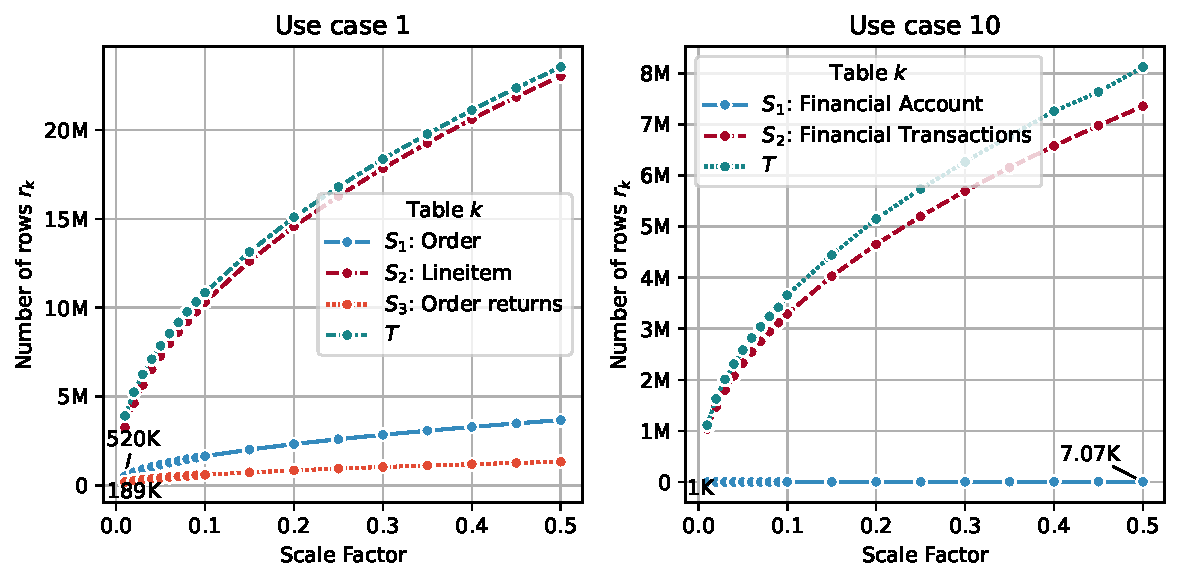
\includegraphics[width=\linewidth]{chapters/06_evaluation/figures/tpcx-ai-data-chars.pdf}
    \caption[TPCx-AI dataset sizes for used scale factors.]{TPCx-AI dataset sizes for used scale factors. The number of columns is independent of the scale factors. For use case 1: $c_1=3, c_2=4, c_3=3, c_T=7$. For use case 10: $c_1=2, c_2=7, c_T=5$.}
    \label{fig:tpcx-ai-data-chars}
\end{figure}


The first use case involves a join operation among three tables. First, the lineitem table is combined with the order returns data, which is subsequently linked with the orders table. This process yields a table with $c_T=7$ columns, with each row representing a product sold in an order. In the TPCx-AI benchmark, customer segmentation is accomplished through KMeans clustering on this dataset. However, we evaluate all four machine learning models outlined in this thesis, focusing on the training procedure rather than the final classifier's effectiveness. The subsequent scenario entails a join between two tables. Here, the transaction table is merged with the customer table, resulting in a table with $c_T=5$ columns aimed at identifying fraudulent transactions. The same models utilized in the first scenario are applied in this context as well. For a complete overview of the dataset schema, including the relevant tables and columns, please refer to \autoref{fig:appendix-tpc-ai-schema}.

\subsection{Hardware}
\label{subsec:6-hardware}
The experiments were conducted on a diverse range of machines to test various hardware configurations. The majority of the experiments were run on the Delft AI Cluster\footnote{\url{https://daic.tudelft.nl/}}, allowing for testing across different GPU architectures. As profiling was not feasible on this cluster, some profiling experiments were carried out on a local machine, AWS, and resources from the Web Information Systems group\footnote{\url{https://www.wis.ewi.tudelft.nl/}}. Details on which experiments were carried out on which specific machines can be found in \autoref{tab:6-hardware-overview}.

\begin{table}[ht]
    \centering
    % LTeX: enabled=false
\begin{tabular}{p{0.15\linewidth}p{0.19\linewidth}p{0.10\linewidth}p{0.20\linewidth}l}
    \toprule
    Experiment type                                                 & Machine                                                         & \hspace{0pt}Architecture                                  & Compute Unit           & Experiment       \\
    \midrule\midrule
    \multirow[t]{3}{*}{\parbox{1\linewidth}{\vspace{1.5cm}profile}} & WIS ST4                                                         & Ampere                                                    & GPU A40                & \texttt{GPU-P-1} \\
    \cline{2-5}
                                                                    & AWS G5.xlarge                                                   & Ampere                                                    & GPU A10G               & \texttt{GPU-P-2} \\
    \cline{2-5}
                                                                    & Personal Workstation                                            & Turing                                                    & GPU 1660Ti             & \texttt{GPU-P-3} \\
    \cline{1-5}
    \multirow[t]{8}{*}{\parbox{1\linewidth}{\vspace{4cm}runtime}}   & \multirow[t]{5}{*}{\parbox{1\linewidth}{\vspace{2cm}DAIC}}      & Ampere                                                    & GPU A40                & \texttt{GPU-T-1} \\

                                                                    &                                                                 & Volta                                                     & GPU V100               & \texttt{GPU-T-2} \\

                                                                    &                                                                 & Pascal                                                    & GPU P100               & \texttt{GPU-T-3} \\

                                                                    &                                                                 & Turing                                                    & GPU 2080Ti             & \texttt{GPU-T-4} \\

                                                                    &                                                                 & Pascal                                                    & GPU 1080Ti             & \texttt{GPU-T-5} \\
    \cline{2-5}
                                                                    & \multirow[t]{3}{*}{\parbox{1\linewidth}{\vspace{2.3cm}WIS ST4}} & \multirow[t]{3}{*}{\parbox{1\linewidth}{\vspace{2.3cm}—}} & EPYC 7H12 CPU 8 cores  & \texttt{CPU-T-1} \\

                                                                    &                                                                 &                                                           & EPYC 7H12 CPU 16 cores & \texttt{CPU-T-2} \\

                                                                    &                                                                 &                                                           & EPYC 7H12 CPU 32 cores & \texttt{CPU-T-3} \\
    \cline{1-5}
    \bottomrule
\end{tabular}

    \caption[Experiment to machine mapping]{Experiment to machine mapping. The experiment type is either profiling or runtime. Profiling experiments are used to collect the hardware specific metrics for our training data. Runtime experiments are used to gather data on the runtime of the factorized ML framework compared to materialized learning.}
    \label{tab:6-hardware-overview}
\end{table}

\subsection{Experiment Setting}
To guarantee the reliability of the training data, each experiment was run with a repetition count of $30$. The profiling experiments, on the other hand, were not replicated, as NCU guarantees consistent and actionable results by replaying kernel launches \cite{nsight_compute}. All experiments were carried out in a containerized setting to ensure reproducibility. The profiling experiments used the same image as the runtime experiments to maintain consistency in the environment. Docker\footnote{\url{https://www.docker.com/}} served as the container runtime, except on the DAIC cluster, where the usage of Apptainer\footnote{\url{https://apptainer.org/}} images was mandated.

\subsection{Validation Strategy}
\label{subsec:6-validation-strategy}
Given the vast range of potential data, model, and hardware features, it is crucial to have confidence in our estimator's ability to provide accurate predictions for new situations. To test this, we implement a rigorous train-validate-test split. $70\%$ of the data from synthetic datasets is allocated to the training set, while the remaining $30\%$ forms the validation set. The real-world datasets are exclusively reserved for testing purposes. Since these datasets are not used in training the cost estimators, they offer a reliable assessment of performance in novel scenarios, as discussed in \autoref{subsec:6-generalizability}. Similarly, to ensure robustness in the hardware aspect, we adopt a comparable strategy by isolating the samples of \texttt{GPU-T-5} for testing. Lastly, to explore the dimension of model characteristics, we perform an ablation study (see \autoref{subsubsec:6-ablation}) to investigate the impact of excluding various models on the cost estimator's performance.

\section{Cost Model Performance and Comparative Analysis}
\label{sec:eval-model-evaluation}

In this section we answer
\begin{itemize}
    \item[RQ.2] How can we accurately predict the optimal choice between factorized or materialized training of a Machine Learning model, on CPU and GPU, through leveraging knowledge about model, data, and hardware characteristics?
\end{itemize}

We first illustrate the comparison of the cost estimators with the state-of-the-art in cost estimation for Factorized Machine Learning training. Next, we demonstrate the ability of the best performing cost estimators to generalize effectively to novel scenarios.

\subsection{Exploring Generalizability}
\label{subsec:6-generalizability}
The aim of this thesis is to create a cost estimator capable of reliably predicting the most suitable option between factorized and materialized training methods for a Machine Learning model. To ensure that this cost estimator maintains good performance in unfamiliar situations, i.e., it is not overfitting to the training data, we evaluate the cost estimators on the real-world datasets, and on new hardware. The results are shown in \autoref{fig:6-generalization}.

\begin{figure}
    \centering
    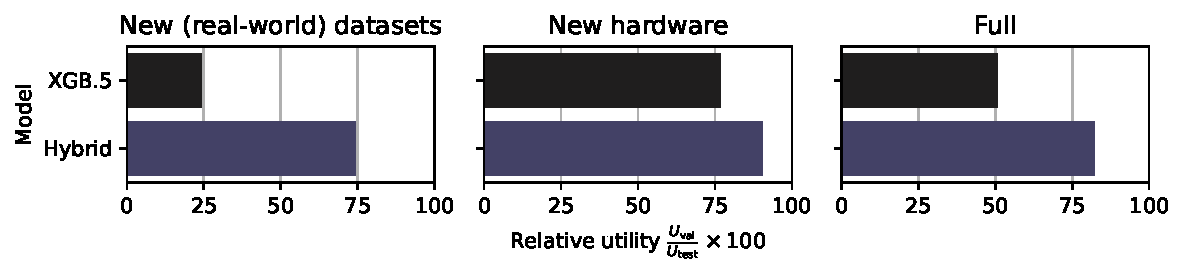
\includegraphics[width=\linewidth]{chapters/06_evaluation/figures/eval_generalization.pdf}
    \caption[Evaluation of utility on new scenarios]{Evaluation and comparison of cost model's relative utility on new scenarios. The x-axis shows the relative utility, defined as total time saved, with regard to the test set, for each group of scenario types. A value of 100\% means that the cost estimator performs equally well on the test set as on the training set. In short, utility is defined as $U = \frac{\text{time saved}}{\text{true time saved}}$. Relative utility shown here is the utility on the validation set (synthetic data) divided by utility on the test set (real-world data): $\frac{U_{\text{val}}}{U_{\text{test}}} \times 100$}
    \label{fig:6-generalization}
\end{figure}

Significant disparities exist among the estimators in terms of their ability to generalize to unfamiliar situations. The analytical models show superior relative utility, which can be attributed to their resistance to overfitting, and their already subpar performance on the training set. The statistical models demonstrate satisfactory relative performance on the real datasets but falter significantly on the new hardware, indicating a failure to adequately capture the relationship between hardware characteristics and cost. The XGBoost models excel in terms of relative performance on new hardware but underperform on the real datasets. The hybrid model combines the strong points of the XGBoost and statistical models, achieving good relative performance of 82\% on the full dataset.

\subsubsection{Ablation Study}
\label{subsubsec:6-ablation}
To assess the generalizability of our cost estimator across new model types, we conduct an ablation study. In this study, we systematically exclude individual model types and assess the estimator’s performance on test set scenarios exclusive to the omitted model type.

\begin{figure}[ht]
    \centering
    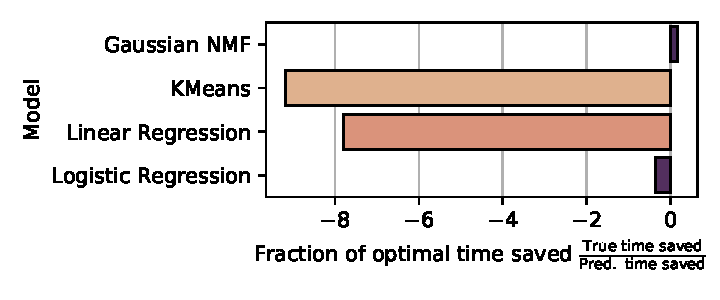
\includegraphics[width=0.6\linewidth]{chapters/06_evaluation/figures/hybrid-ablation.pdf}
    \caption[Results of ablation study]{Result of leave-one-out ablation study. The x-axis shows the relative performance of the cost estimator, defined as total time saved, with regard to the test set, for each group model.}
    \label{fig:6-ablation}
\end{figure}

The results of this ablation study are illustrated in \autoref{fig:6-ablation}. The x-axis represents the relative performance compared to an ideal model. The findings indicate that our hybrid model exhibits suboptimal performance when applied to new model types. While the Gaussian Non-negative Matrix Factorization (NMF) demonstrates marginal utility, facilitating some time savings, the application of our cost estimator to other models, notably KMeans and Linear Regression, would lead to considerable increases in computational time. This suggests that our cost model is specifically tailored to the model types included in its training dataset. The inclusion of linear algebra operators within the training set confers additional benefits, as evidenced in Figure 5 (\autoref{fig:5-xgboost-evaluation}); however, these benefits are insufficient to achieve model independence in cost estimation.

To mitigate this limitation, we propose two potential strategies: First, refining the feature engineering process to incorporate a broader spectrum of model-agnostic derived features, necessitating a comprehensive analysis of the factorized machine learning framework and its supported models. Second, and perhaps more effectively, expanding the training dataset to include emerging models as they are integrated into the factorized machine learning framework.

\subsection{Cost Estimator Comparison}
\label{subsec:6-sota-comparison}
In this section, we evaluate the performance of our cost models with the SOTA. The comparison is based on the same test set used in the previous sections, which includes real datasets and new hardware configurations.

\autoref{fig:6-sota-comparison} presents the results of this comparative assessment. The plot on the left shows the precision, accuracy, f1 score and recall score of the cost estimators. The right plot quantifies the total time saved by the cost estimators across the set of scenarios.

From the figure we can infer how each estimator behaves with regard to the precision/recall trade-off. The SOTA cost estimators show diminished precision, yet augmented recall, indicative of favoring predicting a positive label, which in this case means that the factorized training is faster. MorpheusFI \cite{MorpheusFI} shows the best recall, explained by precision and accuracy, labeling all cases as positive, resulting in a total time loss of $13,000$ seconds. Morpheus \cite{orion_learning_gen_lin_models} presents a lesser time loss of approximately $7000$ seconds, reflecting a slightly more conservative approach than MorpheusFI. Amalur \cite{amalur} shows a total time loss of roughly $500$ seconds, outperforming Morpheus and MorpheusFI. The Hybrid cost estimator introduced in this thesis has a net time savings of $1350$ seconds, with an accuracy of $95\%$, which is a significant improvement over the SOTA.

\begin{figure}[ht]
    \centering
    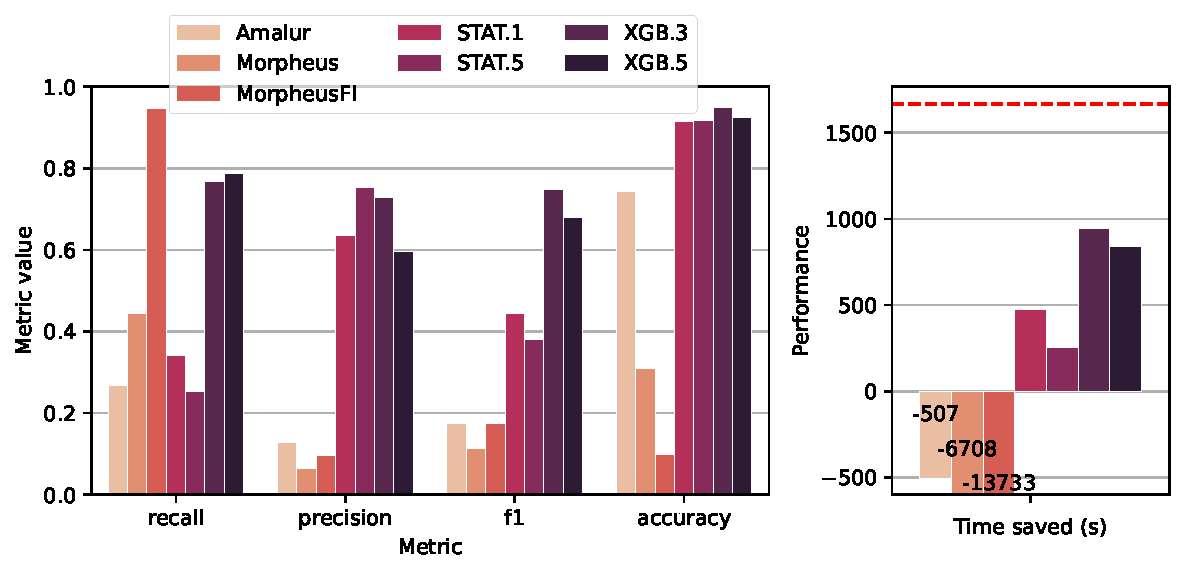
\includegraphics[width=\linewidth]{chapters/06_evaluation/figures/eval_sota_results.pdf}
    \caption[Cost estimator comparison vs. SOTA]{Comparison of the cost estimators. Performance evaluated on the test set (real datasets and new hardware).}
    \label{fig:6-sota-comparison}
\end{figure}

\section{Discussion}
\label{sec:eval-discussion}
We have shown that our hybrid cost estimator is capable of accurately predicting the optimal choice between factorized and materialized training of a Machine Learning model, on both CPU and GPU. The hybrid estimator shows good generalizability to new scenarios and outperforms the SOTA in cost estimation for Factorized ML training. However, there are some limitations to this work.

Our research demonstrates that the Hybrid cost estimator adeptly predicts the most efficient training method -factorized or materialized- for machine learning models across CPU and GPU scenarios. This estimator exhibits commendable generalizability to novel scenarios and surpasses state-of-the-art (SOTA) estimators in the domain of cost estimation for Factorized ML training. However, this study is not without its limitations.

The first important note is that the SOTA cost estimators lack design considerations for GPU-based training. This oversight is non-trivial, as our findings reveal a significant divergence in the factorization-materialization trade-off between CPU and GPU environments.

Another limitation is that the cost estimators were trained on synthetic data. While synthetic data generation aims to replicate real-world datasets, discrepancies with real-world scenarios are inevitable.  Our estimators have demonstrated proficiency with actual data; however, the potential for overfitting to synthetic data cannot be dismissed, and the robust performance observed with datasets such as Hamlet and TPCx-AI may not be entirely indicative of broader applicability. This concern extends to the hardware aspect, where the estimators show promising adaptability to new hardware configurations, yet the question of how representative these configurations are of real-world settings remains uncertain remains.

Despite these limitations, we believe that our contributions to cost estimation for ML training are substantial. The Hybrid cost estimator yields encouraging results and consistently outperforms SOTA in a multitude of scenarios. We hope that this work will inspire continued exploration in this field.

\section{Conclusion}
\label{sec:eval-conclusion}
This chapter has presented the comprehensive evaluation of our hybrid cost estimator for factorized and materialized ML training. We have shown the estimator's ability to accurately discern the optimal training approach and its superiority over SOTA in real-world scenarios. Although the estimator adapts well to new hardware and data parameters, its predictive utility for scenarios involving new ML models is limited.

The next chapter will explore future work and potential improvements for our cost estimator.

